\newcommand{\cryptoMinerTagResultsAucTable}{
    \begin{table}[H]
        \centering
        \begin{tabular}{|p{2,8cm}||P{2,2cm} P{2,2cm} P{2,2cm} P{2,2cm}|}
            \hline
            Crypto-miner Tag & ALOHA\newline (M/B only) & ALOHA & Joint\newline Embedding & Proposed\newline Model \\
            \hline
            AUC-ROC & - & 0.980$\pm$0.003 & 0.986$\pm$0.003 & \textBF{0.990$\pm$0.003} \\
            \hline
        \end{tabular}
        \caption[Crypto-miner Tag prediction task AUC-ROC results]{AUC-ROC (Area Under Curve) of the different models for the \textbf{Crypto-miner Tag} prediction task. Results were aggregated over \textBF{3} training runs with different weight initializations and minibatch orderings. Best results are shown in \textbf{bold}.} \label{tab:cryptoMinerTag_auc}
    \end{table}
}

\newcommand{\cryptoMinerTagResultsAtFprTable}{
    \begin{center}
        \begin{longtable}[c]{|P{3,2cm}||P{1,8cm} P{1,8cm} P{1,8cm} P{1,8cm} P{1,8cm}|}
            \hline
            Crypto-miner Tag & \multicolumn{5}{c|}{{FPR}} \\
            & $10^{-5}$ & $10^{-4}$ & $10^{-3}$ & $10^{-2}$ & $10^{-1}$ \\
            \hline
            \endfirsthead

            \caption*{\raggedright ...continued from previous page} \\
            \hline
            Crypto-miner Tag & \multicolumn{5}{c|}{\textbf{FPR}} \\
            & $10^{-5}$ & $10^{-4}$ & $10^{-3}$ & $10^{-2}$ & $10^{-1}$ \\
            \hline
            \endhead

            \caption*{\raggedleft ...continued on next page} \\
            \endfoot

            \caption[Crypto-miner Tag prediction task results]{Mean and standard deviation results (TPR, Accuracy, Recall, Precision and F1-Score) of the different models for the \textbf{Crypto-miner Tag} prediction task at different \textbf{FPR}s (\textit{False Positive Rates}). Results were aggregated over \textBF{3} training runs with different weight initializations and minibatch orderings. Best results are shown in \textbf{bold}. Under \textbf{TPR} results are also presented the percentage reduction in mean detection error and in ROC curve standard deviation introduced by the \textit{Proposed Model} with respect to both \textit{ALOHA} model and \textit{Joint Embedding}.} \label{tab:cryptoMinerTag_results_at_fpr} \\
            \endlastfoot

            \multicolumn{6}{|c|}{\textbf{TPR}} \\
            \hline
            ALOHA (M/B only) & - & - & - & - & - \\
            ALOHA & 0.136$\pm$0.048 & 0.479$\pm$0.012 & 0.554$\pm$0.014 & 0.773$\pm$0.148 & 0.931$\pm$0.016 \\
            Joint Embedding & 0.266$\pm$0.113 & \textBF{0.522$\pm$0.015} & 0.560$\pm$0.029 & 0.896$\pm$0.008 & 0.961$\pm$0.015 \\
            Proposed Model & \textBF{0.421$\pm$0.045} & 0.505$\pm$0.005 & \textBF{0.565$\pm$0.019} & \textBF{0.905$\pm$0.006} & \textBF{0.966$\pm$0.015} \\
            \hline
            Error Reduction wrt\newline ALOHA (M/B only) & - & - & - & - & - \\
            Error Reduction wrt\newline ALOHA & 33.0\% & 5.0\% & 2.5\% & 58.1\% & 50.7\% \\
            Error Reduction wrt\newline Joint Embedding & 21.1\% & -3.6\% & 1.1\% & 8.7\% & 12.8\% \\
            \hline
            Std Reduction wrt\newline ALOHA (M/B only) & - & - & - & - & - \\
            Std Reduction wrt\newline ALOHA & 6.3\% & 58.3\% & -35.7\% & 95.9\% & 6.3\% \\
            Std Reduction wrt\newline Joint Embedding & 60.2\% & 66.7\% & 34.5\% & 25.0\% & 0.0\% \\
            \hline
            \multicolumn{6}{|c|}{\textbf{Accuracy}} \\
            \hline
            ALOHA (M/B only) & - & - & - & - & - \\
            ALOHA & 0.988$\pm$0.001 & \textBF{0.993$\pm$0.000} & \textBF{0.993$\pm$0.000} & 0.987$\pm$0.002 & 0.900$\pm$0.000 \\
            Joint Embedding & 0.990$\pm$0.002 & \textBF{0.993$\pm$0.000} & \textBF{0.993$\pm$0.000} & \textBF{0.989$\pm$0.000} & \textBF{0.901$\pm$0.000} \\
            Proposed Model & \textBF{0.992$\pm$0.001} & \textBF{0.993$\pm$0.000} & \textBF{0.993$\pm$0.000} & \textBF{0.989$\pm$0.000} & \textBF{0.901$\pm$0.000} \\
            \hline
            \multicolumn{6}{|c|}{\textbf{Recall}} \\
            \hline
            ALOHA (M/B only) & - & - & - & - & - \\
            ALOHA & 0.136$\pm$0.048 & 0.479$\pm$0.012 & 0.554$\pm$0.014 & 0.773$\pm$0.148 & 0.931$\pm$0.016 \\
            Joint Embedding & 0.266$\pm$0.113 & \textBF{0.522$\pm$0.015} & 0.560$\pm$0.029 & 0.896$\pm$0.008 & 0.961$\pm$0.015 \\
            Proposed Model & \textBF{0.421$\pm$0.045} & 0.505$\pm$0.005 & \textBF{0.565$\pm$0.019} & \textBF{0.905$\pm$0.006} & \textBF{0.966$\pm$0.015} \\
            \hline
            \multicolumn{6}{|c|}{\textbf{Precision}} \\
            \hline
            ALOHA (M/B only) & - & - & - & - & - \\
            ALOHA & 0.994$\pm$0.002 & 0.985$\pm$0.000 & 0.886$\pm$0.003 & 0.515$\pm$0.052 & 0.115$\pm$0.002 \\
            Joint Embedding & 0.997$\pm$0.002 & \textBF{0.987$\pm$0.000} & 0.887$\pm$0.006 & 0.556$\pm$0.002 & \textBF{0.119$\pm$0.002} \\
            Proposed Model & \textBF{0.998$\pm$0.000} & 0.986$\pm$0.000 & \textBF{0.888$\pm$0.003} & \textBF{0.559$\pm$0.002} & \textBF{0.119$\pm$0.002} \\
            \hline
            \multicolumn{6}{|c|}{\textbf{F1 Score}} \\
            \hline
            ALOHA (M/B only) & - & - & - & - & - \\
            ALOHA & 0.237$\pm$0.075 & 0.644$\pm$0.011 & 0.682$\pm$0.011 & 0.616$\pm$0.086 & 0.205$\pm$0.003 \\
            Joint Embedding & 0.407$\pm$0.152 & \textBF{0.683$\pm$0.013} & 0.686$\pm$0.024 & 0.687$\pm$0.004 & 0.211$\pm$0.003 \\
            Proposed Model & \textBF{0.591$\pm$0.045} & 0.668$\pm$0.005 & \textBF{0.690$\pm$0.015} & \textBF{0.691$\pm$0.003} & \textBF{0.212$\pm$0.003} \\
            \hline
        \end{longtable}
    \end{center}
}

\newcommand{\cryptoMinerTagResultsSummaryTable}{
    \begin{table}[H]
        \centering
        \begin{tabular}{|P{3,2cm}||P{1,8cm} P{1,8cm} P{1,8cm} P{1,8cm} P{1,8cm}|}
            \hline
            \multicolumn{6}{|c|}{Crypto-miner Tag (at FPR $=1\%$)} \\
            \hline
            Model & TPR & Accuracy & Precision & Recall & F1 score \\
            \hline
            ALOHA (M/B only) & - & - & - & - & - \\
            ALOHA & 0.773$\pm$0.148 & 0.987$\pm$0.002 & 0.515$\pm$0.052 & 0.773$\pm$0.148 & 0.616$\pm$0.086 \\
            Joint Embedding & 0.896$\pm$0.008 & \textBF{0.989$\pm$0.000} & 0.556$\pm$0.002 & 0.896$\pm$0.008 & 0.687$\pm$0.004 \\
            Proposed Model & \textBF{0.905$\pm$0.006} & \textBF{0.989$\pm$0.000} & \textBF{0.559$\pm$0.002} & \textBF{0.905$\pm$0.006} & \textBF{0.691$\pm$0.003} \\
            \hline
        \end{tabular}
        \caption[Summary of Crypto-miner Tag prediction task results]{Summary of the mean and standard deviation results of the different models for the \textbf{Crypto-miner Tag} prediction task at \textbf{FPR} $=1\%$. Results were aggregated over \textBF{3} training runs with different weight initializations and minibatch orderings. Best results are shown in \textbf{bold}.} \label{tab:cryptoMinerTag_result_summary}
    \end{table}
}

\newcommand{\cryptoMinerTagRocAlohaMB}{
    \begin{figure}[H]
        \vspace*{-0.5cm}
        \centering
        \includegraphics[width=0.6\textwidth]{./results/crypto_miner_tag_roc_alohaMB.png}
        \vspace*{-0.2cm}
        \caption[Crypto-miner Tag prediction task ALOHA (M/B only) ROC curve]{ROC curve and AUC statistics of \textBF{ALOHA (M/B only)} model for the \textbf{Crypto-miner Tag}. The line represents the \textit{mean} TPR at a given FPR, while the shaded region represents the \textit{standard deviation}. Statistics were computed over \textBF{3} training runs, each with random parameter initialization.}
        \label{fig:cryptoMinerTagRocAlohaMB}
    \end{figure}
}

\newcommand{\cryptoMinerTagRocAloha}{
    \begin{figure}[H]
        \vspace*{-0.5cm}
        \centering
        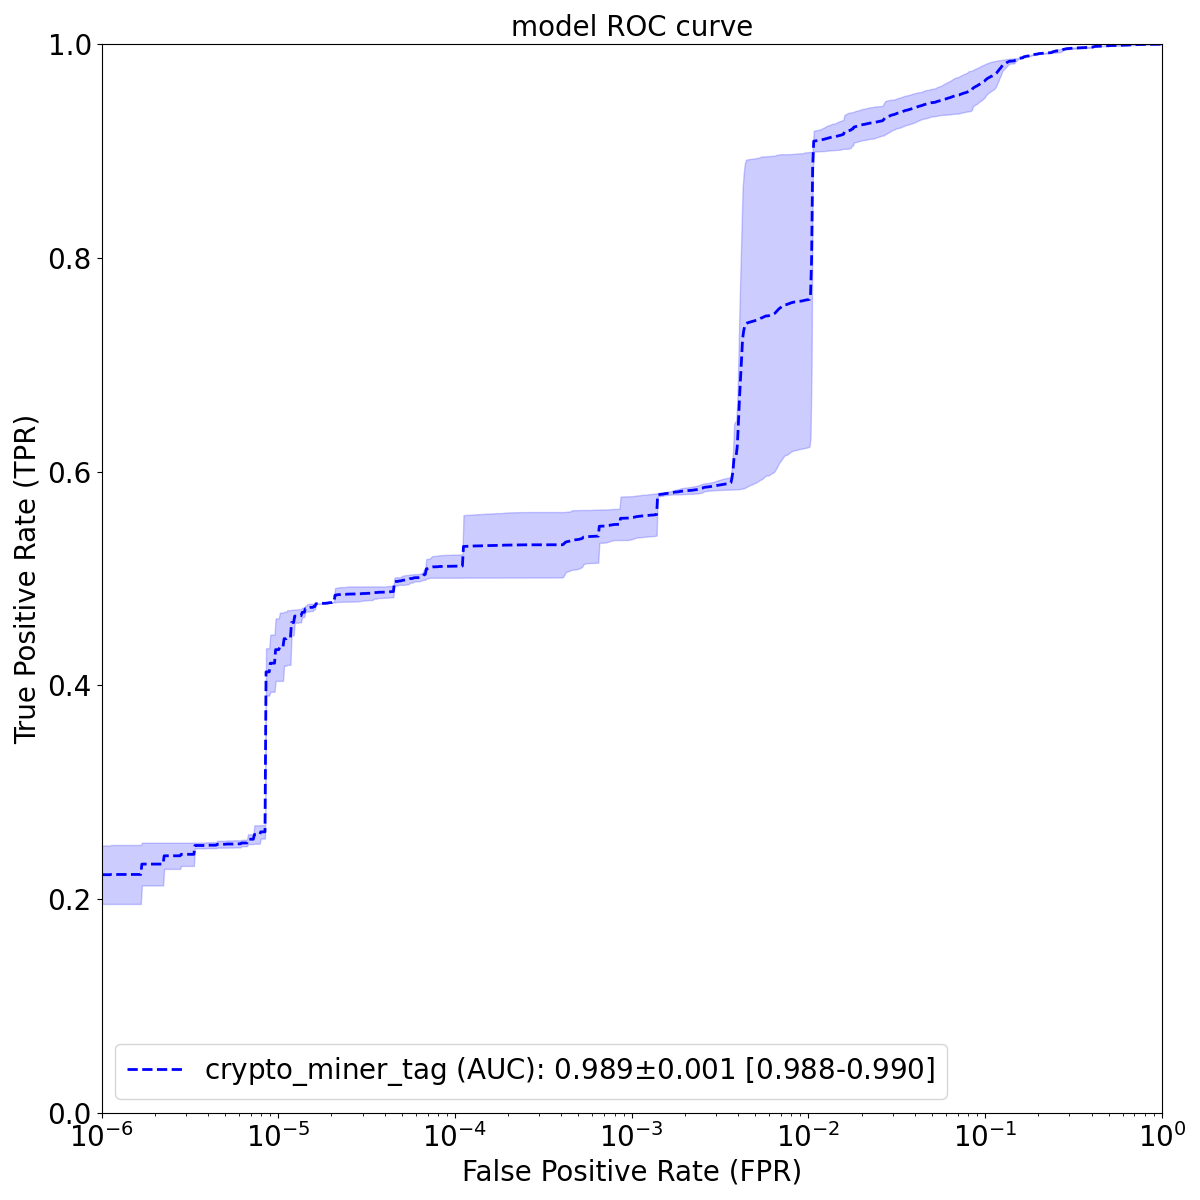
\includegraphics[width=0.6\textwidth]{./results/crypto_miner_tag_roc_aloha.png}
        \vspace*{-0.2cm}
        \caption[Crypto-miner Tag prediction task ALOHA ROC curve]{ROC curve and AUC statistics of \textBF{ALOHA} model for the \textbf{Crypto-miner Tag}. The line represents the \textit{mean} TPR at a given FPR, while the shaded region represents the \textit{standard deviation}. Statistics were computed over \textBF{3} training runs, each with random parameter initialization.}
        \label{fig:cryptoMinerTagRocAloha}
    \end{figure}
}

\newcommand{\cryptoMinerTagRocJointEmbedding}{
    \begin{figure}[H]
        \vspace*{-0.5cm}
        \centering
        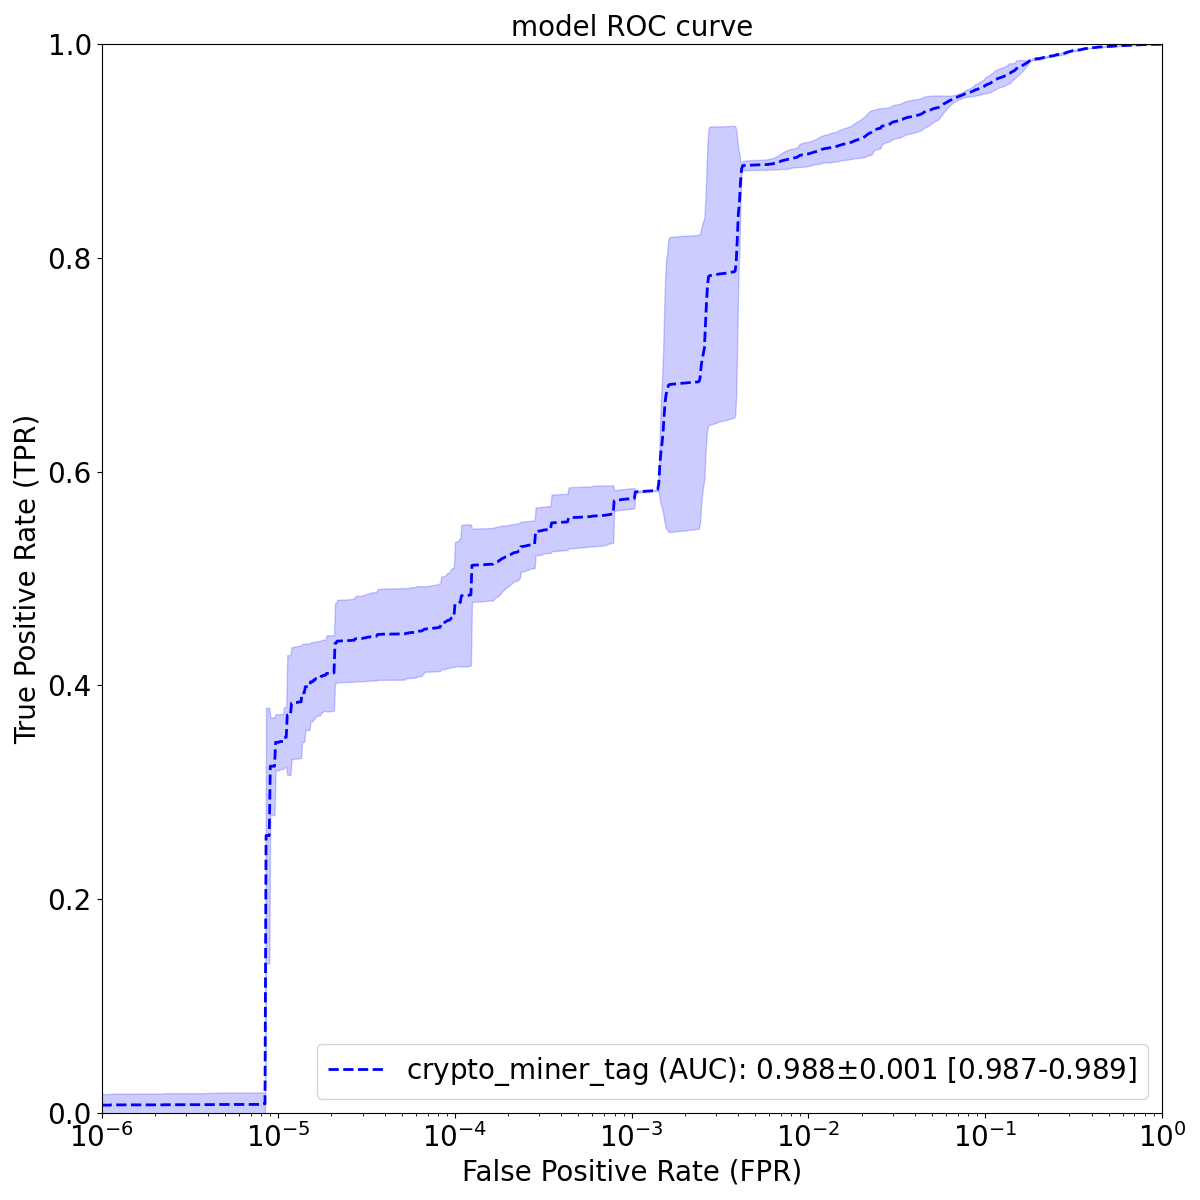
\includegraphics[width=0.6\textwidth]{./results/crypto_miner_tag_roc_jointEmbedding.png}
        \vspace*{-0.2cm}
        \caption[Crypto-miner Tag prediction task Joint Embedding ROC curve]{ROC curve and AUC statistics of \textBF{Joint Embedding} model for the \textbf{Crypto-miner Tag}. The line represents the \textit{mean} TPR at a given FPR, while the shaded region represents the \textit{standard deviation}. Statistics were computed over \textBF{3} training runs, each with random parameter initialization.}
        \label{fig:cryptoMinerTagRocJointEmbedding}
    \end{figure}
}

\newcommand{\cryptoMinerTagRocProposedMethod}{
    \begin{figure}[H]
        \vspace*{-0.5cm}
        \centering
        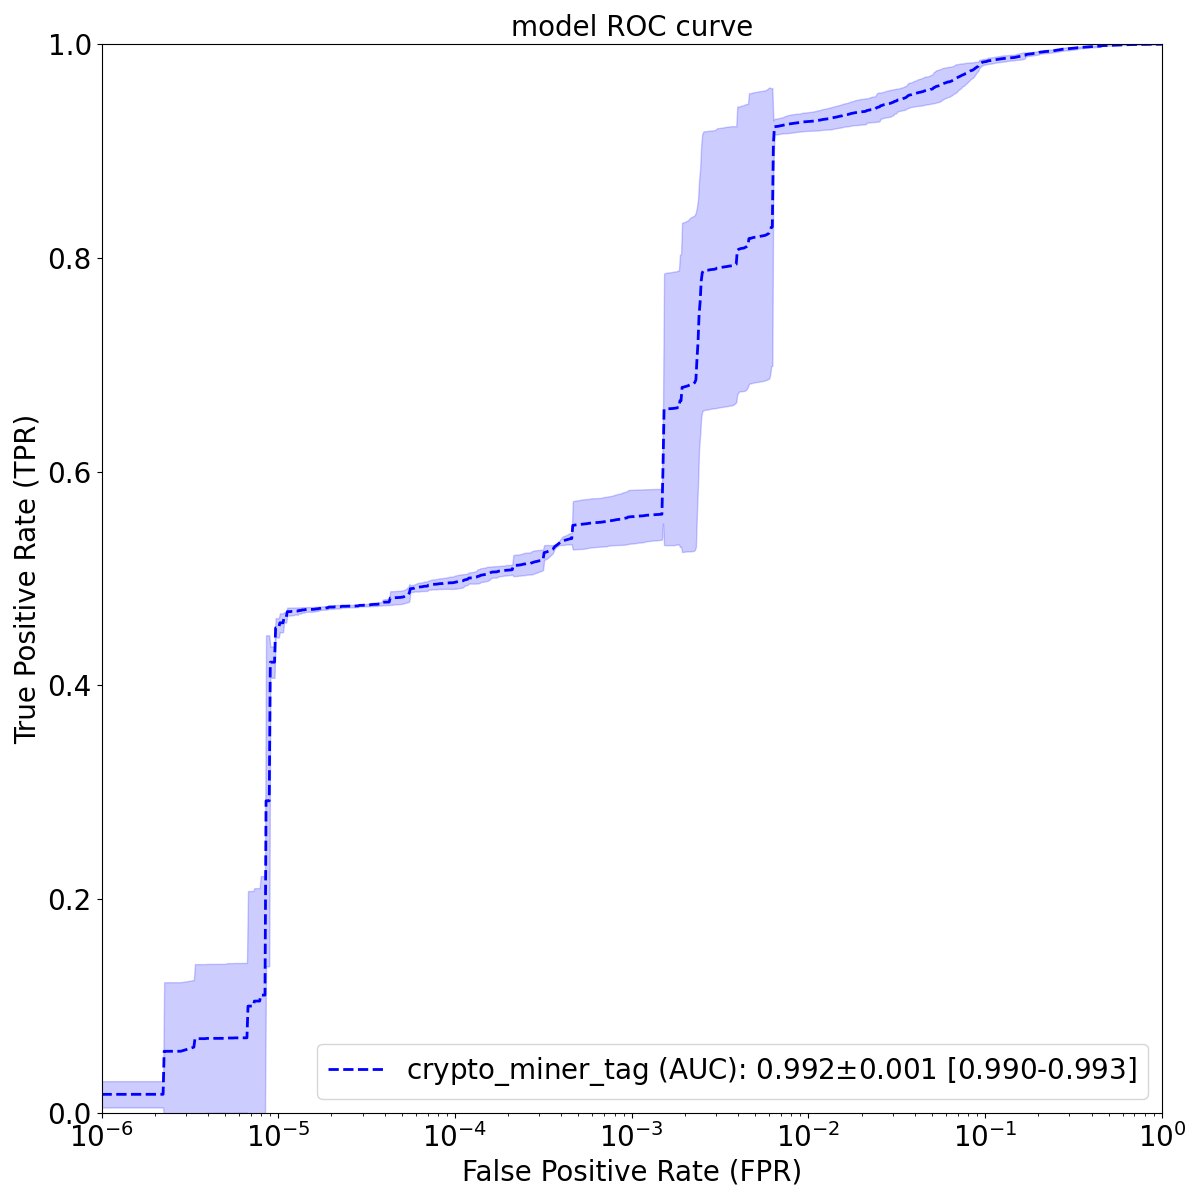
\includegraphics[width=0.6\textwidth]{./results/crypto_miner_tag_roc_proposedModel.png}
        \vspace*{-0.2cm}
        \caption[Crypto-miner Tag prediction task Proposed Model ROC curve]{ROC curve and AUC statistics of \textBF{Proposed Model} for the \textbf{Crypto-miner Tag}. The line represents the \textit{mean} TPR at a given FPR, while the shaded region represents the \textit{standard deviation}. Statistics were computed over \textBF{3} training runs, each with random parameter initialization.}
        \label{fig:cryptoMinerTagRocProposedModel}
    \end{figure}
}
